%!TEX root = ../thesis.tex
%*******************************************************************************
%*********************************** Second Chapter *****************************
%*******************************************************************************
\chapter{Introduction to wind turbine modeling and design}
%*******************************************************************************
\hfill
\localtableofcontents
\newpage



%https://eolienne.f4jr.org/eolienne_etude_theorique

%https://www.geotechnique-journal.org/articles/geotech/pdf/2018/04/geotech190004s.pdf

%https://en.wikipedia.org/wiki/Wind-turbine_aerodynamics

%@book{hansen2015aerodynamics,
%  title={Aerodynamics of wind turbines},
%  author={Hansen, Martin OL},
%  year={2015},
%  publisher={Routledge}
%}

%============================================================%
%============================================================%
\section{Introduction}
%============================================================%
%============================================================%

Wind energy is a highly competitive industry with increasing regulations regarding its impact on ecosystems, land-use conflicts, landscapes, or air traffic management \citep{eolien_en_mer_2022}. 
During the long process to win calls for tenders, obtain construction permits, or throughout the wind farm exploitation, an advanced technical understanding of such systems might offer a competitive advantage. 

The operation of offshore wind turbines are driven by multiple physics coupled. 
This behavior results from different external solicitations which are highly turbulent and uncertain. 
Among them, the \textit{metocean} (abbreviation of meteorology and oceanography) environmental conditions play an important role. 
Note that many other types of solicitations also affect the exploitation of offshore wind turbines (e.g., corrosion of the structure, global scour, marine growth, stress concentration factor induced by the manufacturing quality, etc.). 

In this context, numerical models have been developed to certify the structural integrity of OWTs with respect to their solicitations. 
A wind farm project planned at given location should pass different validation procedures established by international standards such as the International Electrotechnical Commission \citep{iec_2019}. 
As wind turbine structures face a large amount of stress cycles in their lifetime (up to $10^8$ for 25 years of operation), this chapter will particularly focus on fatigue damage assessment.


This chapter briefly introduces wind turbine modeling and design, in the following layout: 
Section \ref{sec:metocean_simulation} presents the methods used for wind and wave generation and wake simulation at a farm scale; 
Section \ref{sec:owt_modeling} recalls elements of theory associated with wind turbine modeling; 
Section \ref{sec:owt_design} introduces recommended practices regarding design and operation;
finally, Section \ref{sec:owt_uncertainties} gives a description of the various sources of uncertainties considered in this thesis. 
Considering the standard uncertainty quantification diagram presented in \fig{fig:UQ_methodo}, the material of this chapter is related to the step A (problem specification) and the step B (uncertainty quantification). 
%To go further this general introduction, the reader might refer to the following sources on the different topics 



%============================================================%
%============================================================%
\section{Metocean conditions simulation} \label{sec:metocean_simulation}
%============================================================%
%============================================================%

In the atmosphere, the wind is the air movements caused by the heterogeneous solar heating of Earth's surface. 
Winds usually move from high-pressure to low-pressure regions. 
Earth's rotation also impacts large-scale climate patterns, including winds, according to the well-known Coriolis effect. 
The wind is a highly variable resource, making its exploitation for energy production uncertain. 
This variability is both expressed in space and time with different behaviors depending on the scales studied. 

Regarding large timescales, yearly seasonal fluctuations of wind conditions are well-defined using probability distributions (typically Weibull distributions). 
Predictions at a shorter timescale are usually unreliable beyond a few days ahead. 
Under a few days, the spectral wind energy distribution per time unit is repesented by its power spectral density (PSD). 
Historically, the spectral study of horizontal wind by \citet{van_1957_wind_psd} for timescales between a few seconds and ten days revealed distinct ranges of behaviors. 
The PSD, such as the one illustrated in \fig{fig:wind_psd}, presents three main separated peaks, explaining how the wind energy is split. 
The two first peaks are named ``synoptic'' and ``diurnal'' peak, which respectively correspond to return periods around four days and one day.
While these two peaks are relatively close together, the third peak is completely separated. 
This peak describes the energy related to the wind turbulence, which evolves in the range below ten minutes. 
Considering this energy distribution, wind behaviors are often referred to as ``short-term'' (for turbulent wind) and ``long-term'' (otherwise). 
In wind turbine simulation, ten minutes simulations became a common practice to fully consider turbulent winds. 

Note that the spectrum presented in the research paper of \citet{van_1957_wind_psd} was build from wind measures near New York, USA. 
The same pattern between the three peaks is rather constant between sites, however, the geography (including the surface roughness, the topology, the proximity to the coast, etc.) may affect this distribution. 
At a larger timescale than one year, assessing trends becomes complicated. 
Wind resource assessment over decades are made more uncertain by the human-caused climate change \cite{nagababu_2023_climate_change}, which disrupts large weather trends and the occurrence of extreme events. 

\begin{figure}
    \centering
    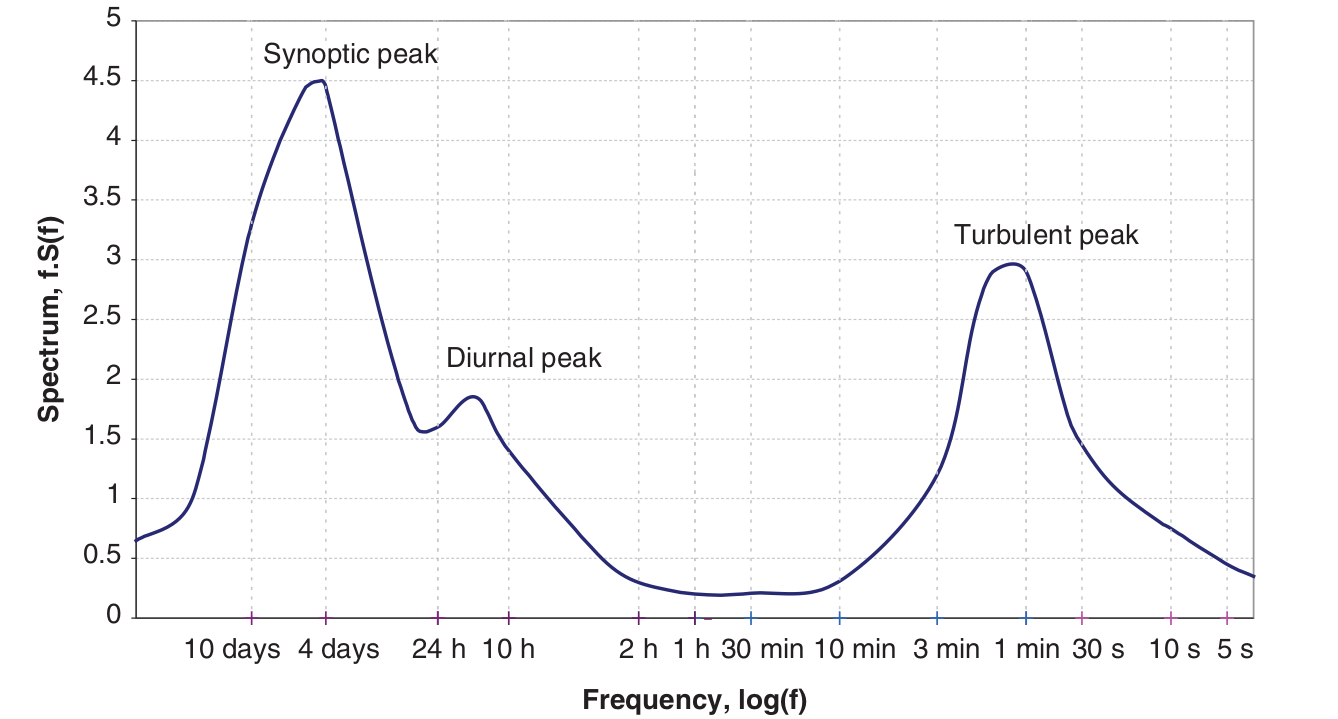
\includegraphics[width=0.7\textwidth]{./part1/figures/wind_spectrum.png}
    \caption{Wind spectrum from Brookhaven, USA (source: \citet{burton_2021_wind_handbook})}
    \label{fig:wind_psd}
\end{figure}


\noindent
\elias{Add something general regrading wave modeling?}



%============================================================%
\subsection{Turbulent wind generation}
%============================================================%

The wind turbulence is a complex and aleatory process, often described as chaotic, since a small perturbation of its initial conditions might have an important impact on the response. 
However, the wind over short-term periods (i.e., ten minutes periods) is usually assumed to be a Gaussian process with constant mean $\overline{U}$ and standard deviation $\sigma_U$ \citep{burton_2021_wind_handbook}. 
Its mean is modeled by the long-term wind conditions (i.e., mean wind speed), often described by a probabilistic model such as a Weibull distribution. 
Note that this assumption is based on the bimodal wind energy distribution observed in \fig{fig:wind_psd}, which might vary at some specific locations. 

The \textit{turbulence intensity} is a commonly used normalized statistic of the wind variability: 
\begin{equation}
    I = \frac{\sigma_U}{\overline{U}}.
\end{equation}

\begin{figure}
    \centering
    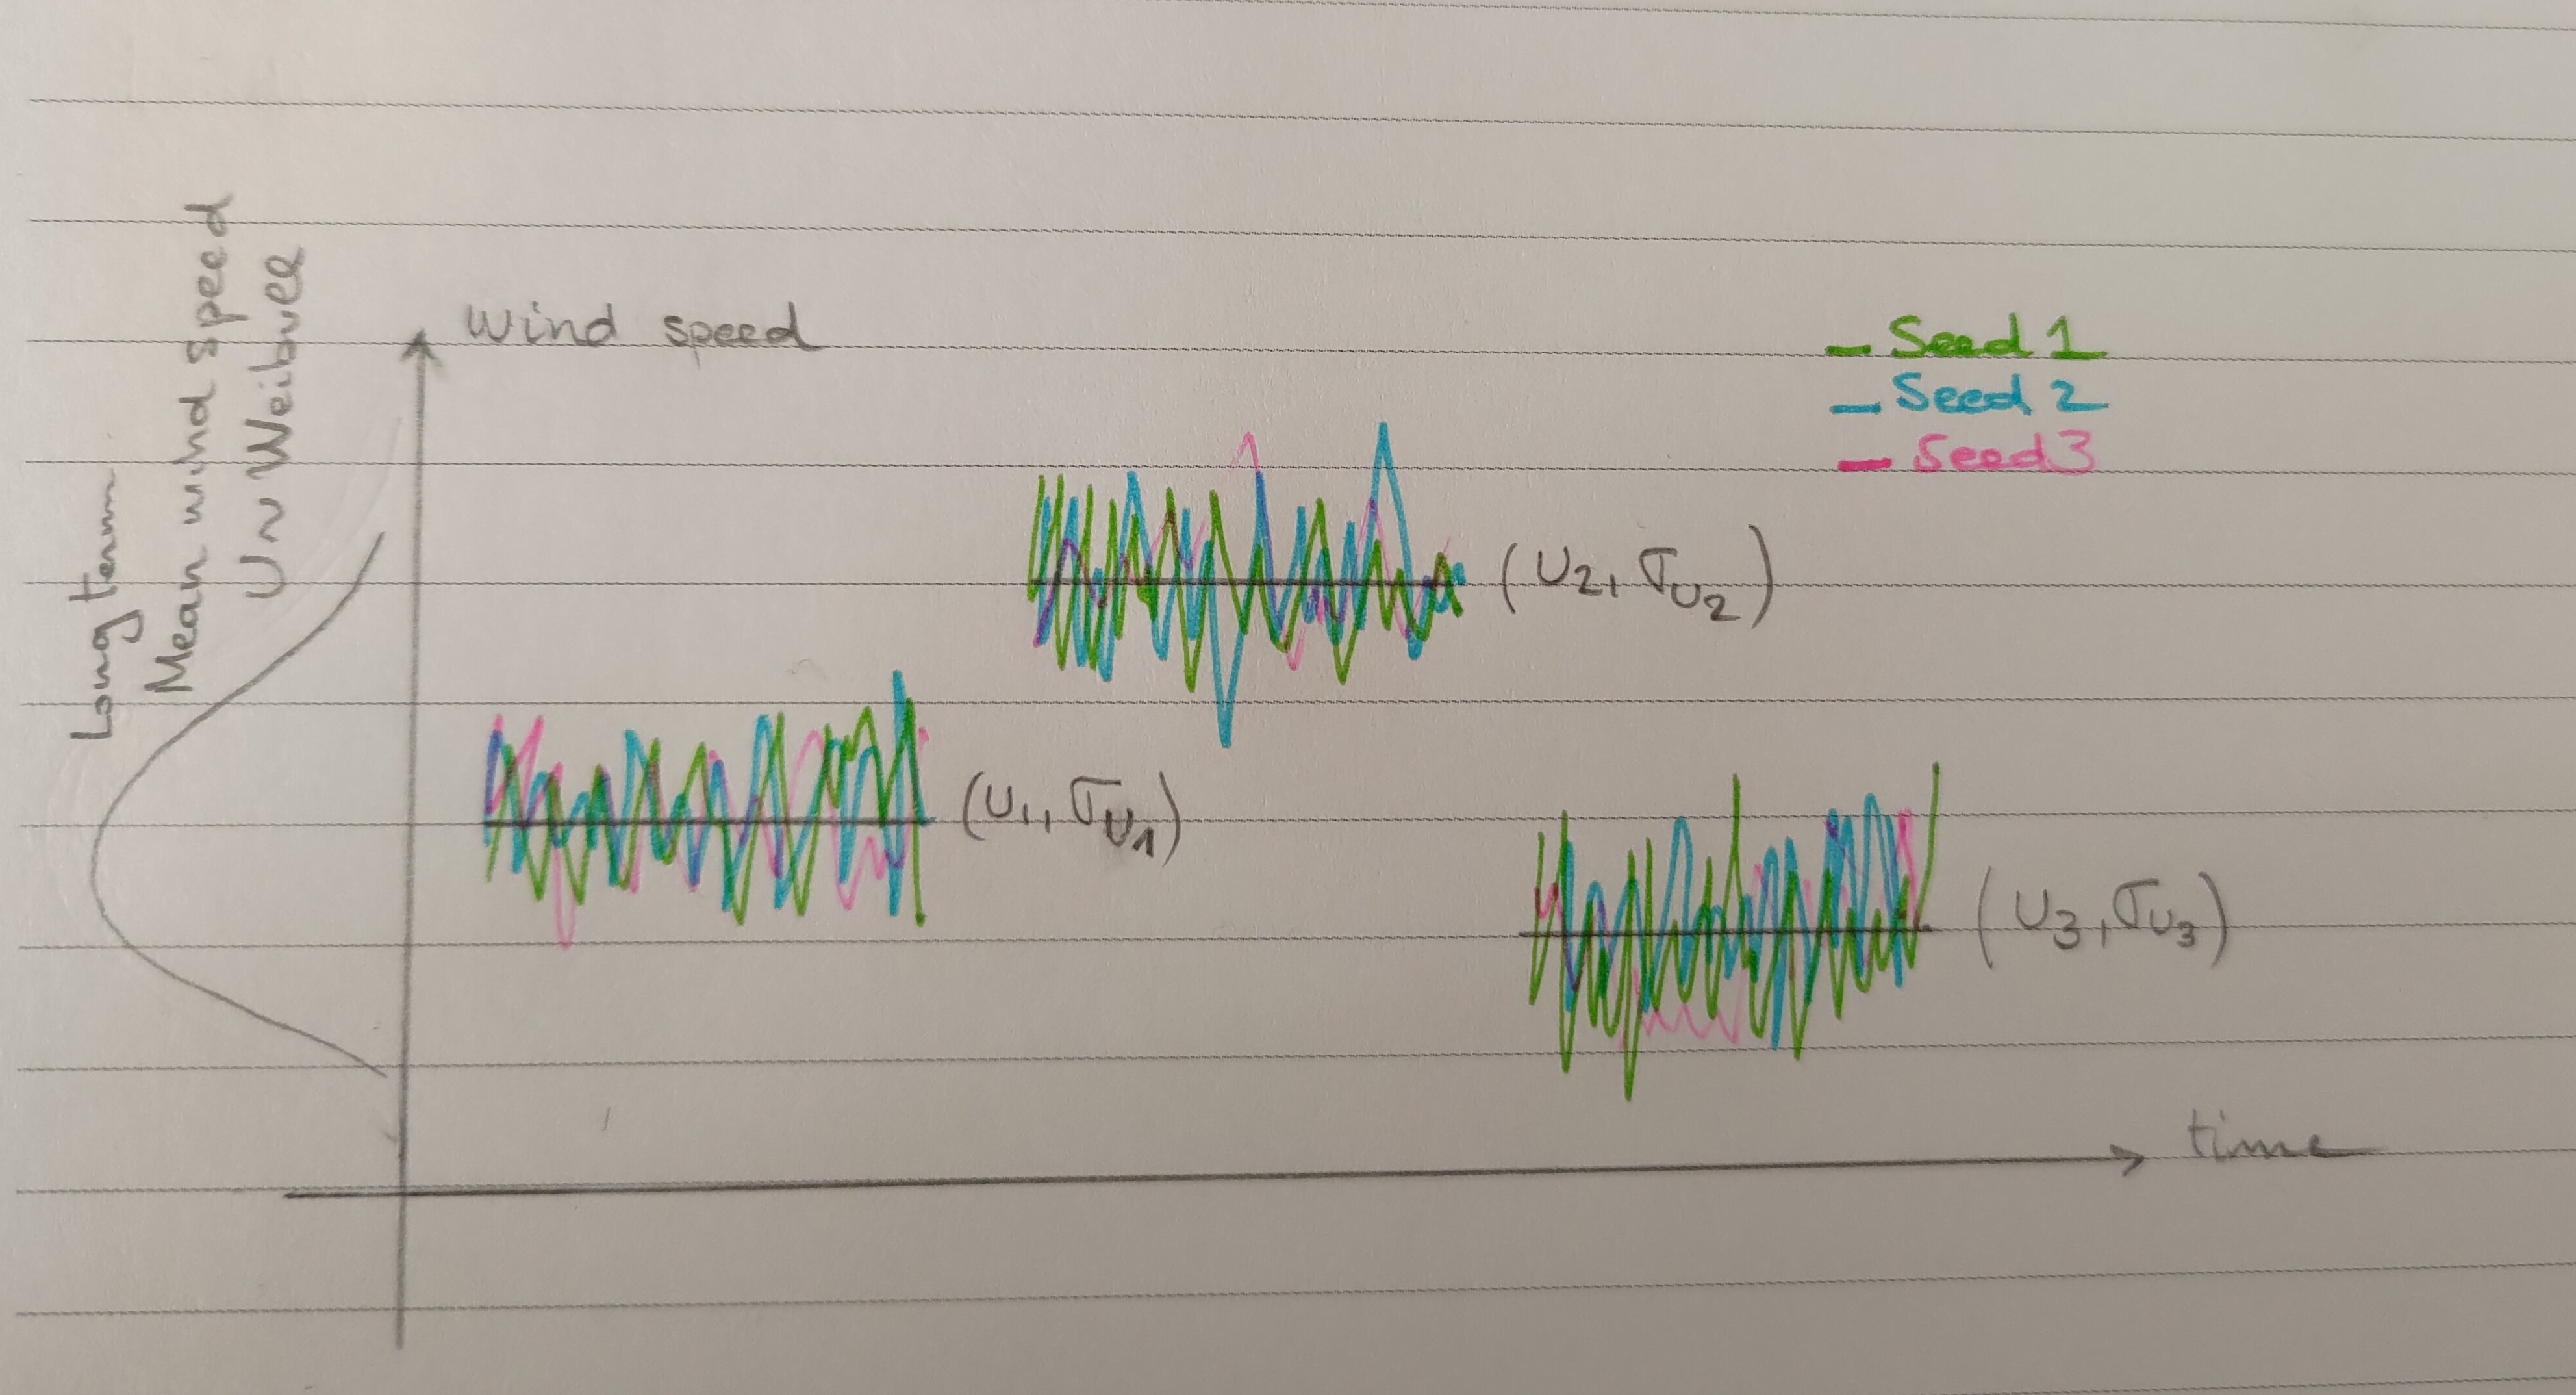
\includegraphics[width=0.7\textwidth]{./part1/figures/wind_long_short_term.jpg}
    \label{fig:wind_long_short_term}
    \caption{\elias{Representation to be confirmed and mentioned in the text}}
\end{figure}

As the wind depends on differences between pressure, humidity, air density, different models exist to represent vertical wind profiles. 
The vertical change in wind conditions is referred to as \textit{vertical wind shear}.
Assuming a constant standard deviation over the altitude, the power law is a widely used approximated shear model \citep{iec_2019}:
\begin{equation}
    \overline{U}(z) = \overline{U}_0 \left(\frac{z}{z_{\mathrm{0}}}\right)^\alpha,
\end{equation}
with $\overline{U}_0$ a well-defined mean wind speed at the height $z_{\mathrm{0}}$ (typically corresponding to a measurement height), 
$z$ the studied height (e.g., the turbine's hub-height), and $\alpha$ the vertical shear coefficient (defined according to measures or standards recommendations). 

To generate a turbulent wind field on a mesh around the turbine, the general mechanism is to apply inverse Fourier transforms on a turbulent wind spectrum.  
Two types of parametric spectrums are commonly used in wind energy: the \textit{Kaimal model} \citep{kaimal_1972} and the \textit{Mann model} \citep{mann_1998}. 
In this thesis, the Kaimal spectrum as defined in \cite{iec_2019} is used for turbulent wind generation over the Cartesian component $k \in \{u, v, w\}$:
\begin{equation}
    S_k(f) = \frac{4 \sigma_k^2 \frac{L_k}{\overline{U}}}{\left(1 + 6 f \frac{L_k}{\overline{U}}\right)^{5/3}},
    \label{eq:kaimal}
\end{equation} 
such that $f$ is the frequency, $\overline{U}$ is the longitudinal mean speed at hub-height, $L_k$ are the Kaimal length scales, and $\sigma_k$ standard deviations (see the complete definition in Annex C of \cite{iec_2019}). 
Along with the Kaimal wind speed spectrum, a spacial coherence model is usually defined in the frequency domain. 
Each couples of nodes in the mesh are correlated, for example, using an exponential coherence model (for further detail in Annex C from \cite{iec_2019}).

In this thesis, the full-field turbulent wind fields (i.e., over a regular mesh) are generated using TurbSim, a software developed by the National Renewable Energy Laboratory (NREL) \citep{turbsim_2009}. 
TurbSim generates time realizations by adapting the spectral method proposed in \citet{veers_1988_sandia} (relying on the inverse Fourier transforms of each component).   
Considering a wind spectrum (e.g., Kaimal model) and a vertical shear model (e.g., power law), TurbSim takes as inputs a mean wind speed, a turbulence standard deviation and a mean wind orientation. 
\fig{fig:turbsim_simu} illustrates the corresponding wind field generated by a ten-minutes TurbSim simulation, considering a set of input long-term conditions. 

\begin{figure}
    \centering
    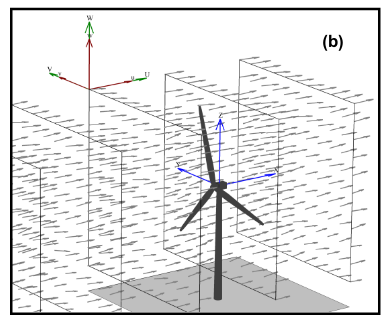
\includegraphics[width=0.5\textwidth]{./part1/figures/turbsim.png}
    \caption{Example of a turbulent wind field generated by TurbSim (source: \citet{turbsim_2009})}
    \label{fig:turbsim_simu}
\end{figure}

In their recent review of the challenges in wind energy, \citep{veers_2019_review} list some limits of the two spectral turbulence models recommended by the standards. 
First, their parameters were fitted using a restricted amount of data \citep{dimitrov_2017_turbulence_models_on_loads}. 
Second, the spacial coherence models associated with Kaimal models showed differences with turbulence measured on site \citep{saranyasoontorn_2004}.  
Finally, recent studies showed that the choice of spectral model impacts the resulting wind turbines loads \citep{doubrawa_2019}. 
These approximations generally tend to overestimate wind flows, leading to conservative designs.

To ensure the most realistic turbulent wind field generation, two research perspectives are actively explored. 
Authors recently developed hybrid methods, including measurement data to enhance spectral models \citep{dimitrov_2017_constrained_turbulence}. 
Alternatively, higher fidelity models were studied in this domain, see for example the use of vortex methods \citep{branlard_2017_book} and large eddy simulations (LES) \citep{doubrawa_2019,bui_2022_mesoscale_LES}.  
Such complex models allow the simulation of mesoscale conditions (e.g., at the farm scale), and extreme transient events (e.g., gusts and storms). 
However, their computational cost is often prohibitive in uncertainty quantification studies. 
When studying the wind resources at a wind farm scale, modeling wind energy losses induced by the turbines' wake becomes essential.


%============================================================%
\subsection{Wake modeling}
%============================================================%

The wake is caused by the wind energy extraction, reducing the wind speed and increasing the turbulence downstream of the turbines (see the illustration in \fig{fig:wake_illustration}). 
In a wind farm, this effect depends on the spacing between turbines, as well as the ambient wind speed and turbulence intensity. 
The turbines positioned at the center of the farm are the most impacted by the wake. 
As a wind farm owner, the consequence of the wake is twofold: a loss of energy production (in the range of 10 to 20 percents depending on the farm), and an increase of fatigue loads (due to the asymmetric loading from the created turbulences).

\begin{figure}
    \centering
    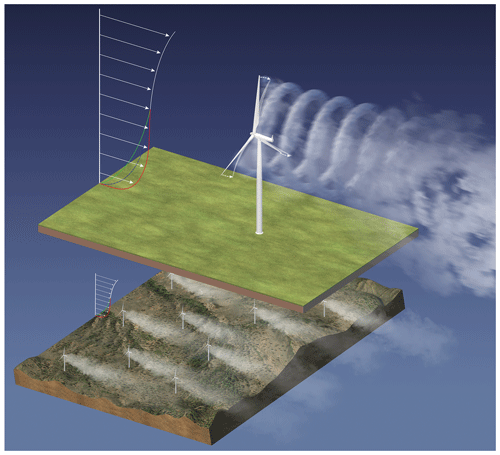
\includegraphics[width=0.5\textwidth]{./part1/figures/wake.png}
    \caption{Illustration of the wake created downstream a wind farm (source: \citet{veers_2019_review})} 
    \label{fig:wake_illustration}
\end{figure}

The initiation of the wake is a complex physical mechanism, however, the wake almost becomes axisymmetric after two turbine diameters downstream. 
At this stage, the wind speed deficit often presents a Gaussian profile centered on the hub \citep{burton_2021_wind_handbook}. 
Numerical models of different fidelities aim at simulating the wake. 
For example, computational fluid dynamics (CFD) models give a detailed description of the wake (including near the turbine) but require high computational efforts. 
In practice, simple analytical models (often called ``engineering models'') are widely used and recommended by standards (see e.g., Annex E in \citet{iec_2019}). 
These models mostly rely the equivalence between the thrust load on the turbine wind energy deficit. 
Since the seminal engineering model proposed by \citet{jensen_1983_wake}, multiple enhancements were proposed. 
A wide benchmark of the wake modeling solutions for different fidelities was performed in \citet{doubrawa_2020_benchmark} and \citet{hiperwind_2023_wp3}. 
The optimal tuning of these engineering models was studied using measurements from a Doppler wind lidar in \citet{zhan_2020_optimal_wake}. 
Different software programs propose wake engineering models, such as: FLORIS (developed by the NREL \citet{fleming_2020_FLORIS}), FarmShadow (developed by IFPEN). 

To take into account the wake effect, control strategies increasingly move from the turbine scale to the farm scale. 
This concept, called ``active wake control'', introduces small yaw misalignments (making the control of turbines individually suboptimal) to optimize the global wake inside the farm \citep{rott_2018_active_control,simley_2020_active_control}. 


%============================================================%
\subsection{Irregular wave generation}
%============================================================%

The propagation of wind generated waves has long been studied in hydrodynamics, leading to various wave theories including Airy's, and Stokes'. 
Airy wave theory (also referred to as linear wave theory), models sea states under the hypothesis of small waves relatively to the water depth.  
This spectral approach superposes many regular waves, following the same wave spectrum, to model irregular waves. 
Standard statistics are used in oceanography to represent sea states and their corresponding wave spectra: 
the wave period $T_p$ (with respective frequency $f_p$), and the significant wave height $H_s$ (average over the highest third of the waves measured). 

The most commonly used parametric wave spectrum is called JONSWAP, after the Joint North Sea Wave Project \citep{jonswap_1973}: 
\begin{equation}
    S(f) = \delta \frac{H_s^2}{f} \left(\frac{f_p}{f}\right)^4 \exp\left[-\frac54 \left(\frac{f_p}{f}\right)^4 \right] \gamma^\alpha.
    \label{eq:jonswap}
\end{equation}
The JONSWAP spectrum is a correction of the Pierson-Moskowitz spectrum, adding the peak enhancement factor $\gamma^\alpha$. 
Further details regarding the numerical values to choose in \eq{eq:jonswap} are given in \citet{burton_2021_wind_handbook}. 
An illustration of the two spectra is presented in \fig{fig:jonswap}, revealing the artificial enhancement factor proposed in the JONSWAP model to better fit sea states measurements. 

\elias{Add elements from E.Petrovska p.13 regarding bimodal spectra}


\begin{figure}
    \centering
    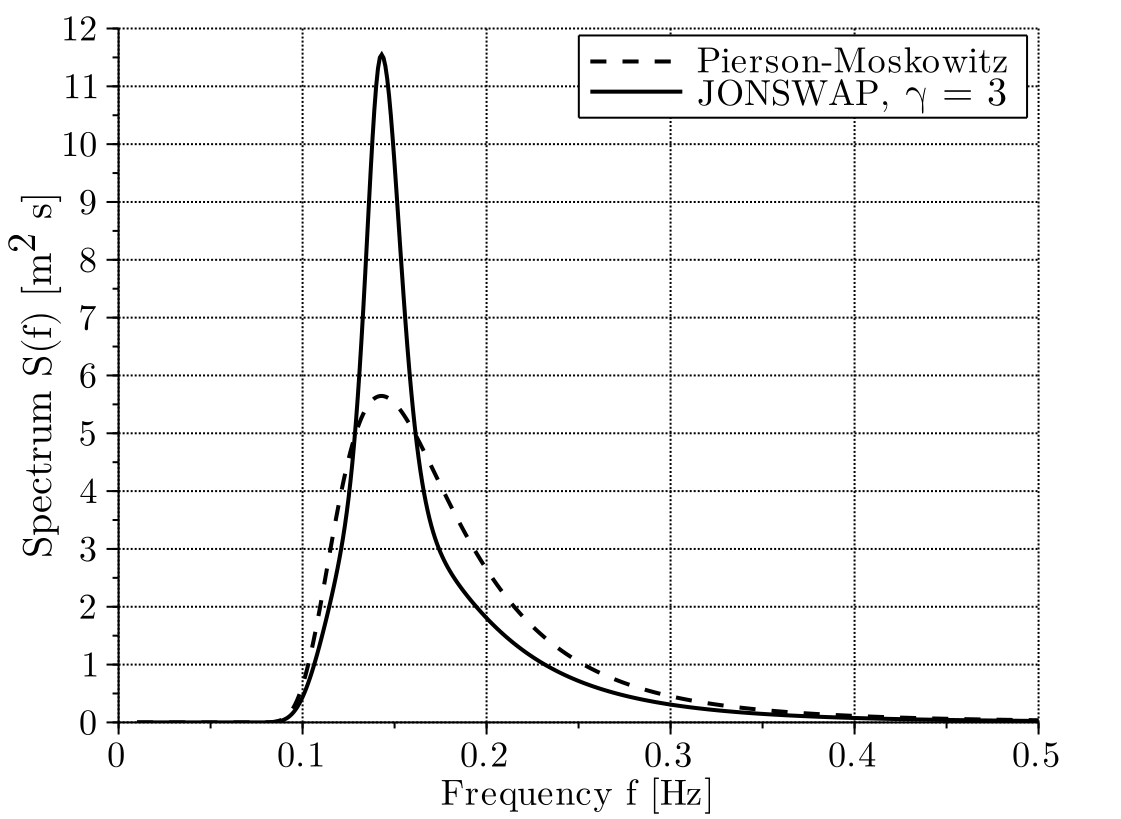
\includegraphics[width=0.5\textwidth]{./part1/figures/jonswap.png}
    \caption{Peirson-Moskowitz and JONSWAP spectra at significant wave height $H_s = 3$
    m and peak period $T_p = 7$ s (source: \citet{milano_thesis_2021})}
    \label{fig:jonswap}
\end{figure}




%============================================================%
%============================================================%
\section{Wind turbine multi-physics modeling} \label{sec:owt_modeling}
%============================================================%
%============================================================%

Offshore wind turbine models are coupling multiple physics such as aerodynamics, hydrodynamics, mechanical elasticity, control and mooring dynamics for floating OWT. 
Similarly to the usual practices from the offshore oil \& gas industry, OWT have been first modeled in the frequency domain. 
At an early design stage, a study in the frequency domain gives a rough idea of the system's feasibility by computing its natural frequencies. 
An OWT should not have its natural frequencies in the same range as the main frequencies of the wave energy spectra. 
Otherwise, such systems can be subject to critical dynamic resonance, leading to their failure.

Beyond this preliminary check, frequency-domain approaches present limits for OWT modeling. 
As they rely on linear assumptions, they are unable to model the non-linearities and transient loading phases \citep{matha_2011_ISOPE}. 
These aspects happen to be essential in the design of OWT \citep{jonkman_2011_ISOPE}. 
As an alternative, the behavior of OWT systems are also simulated in the time domain. 

In the time domain, such systems may be models at different fidelities. 
The diagram in \fig{fig:owt_modeling_fidelities}, illustrates the increasing complexities for two physics involved in OWT modeling (aerodynamics and structural dynamics). 
To perform an uncertainty quantification around a wind turbine model, its fidelity is preferably low. 
At the wind turbine scale, the numerical model studied in this work is actually a chain of three models executed sequentially. 
Note that the wake should also be considered at the wind farm scale, as described earlier. 

\begin{figure}
    \centering
    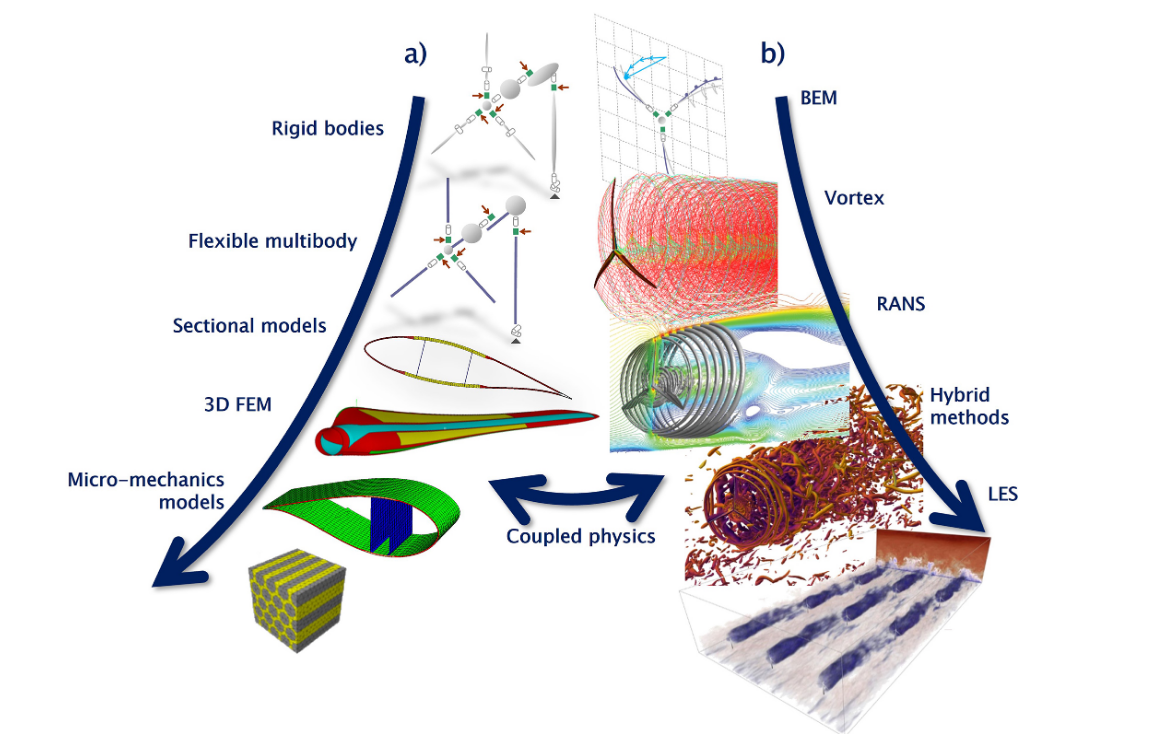
\includegraphics[width=0.7\textwidth]{./part1/figures/OWT_modeling_fidelities.png}
    \caption{Hierarchy of structural (a) and aerodynamic (b) wind energy systems models (source: \citet{veers_2019_review})}
    \label{fig:owt_modeling_fidelities}
\end{figure}


%============================================================%
\subsection{Aerodynamics of horizontal axis wind turbines}
%============================================================%

The structural response...

%============================================================%
\subsection{Hydrodynamics}
%============================================================%


%============================================================%
\subsection{Command and control}
%============================================================%


%============================================================%
\subsection{Structural dynamics}
%============================================================%


%============================================================%
\subsection{Fatigue damage}
%============================================================%





%============================================================%
%============================================================%
\section{Design and operation practices} \label{sec:owt_design}
%============================================================%
%============================================================%

Generally speaking, the energy available in the wind is proportional to the cube of the wind speed, given the well-known power production equation:
\begin{equation}
    P = \frac12 C_p \rho A U^3,
\end{equation}  
where \elias{continue the description}.


%============================================================%
\subsection{Wind turbine design and operation}
%============================================================%
    \begin{itemize}
        \item Different parts of the turbine (monopile, transition piece, fundation, tower), different turbine designs
        \item What are the key steps for a wind farm project in France 
        \item Pre-installation measures are usually done for a period of 1 to 3 year. This data is often validated against long-term regional datasets \cite{sempreviva_2008_wind_assessment_review}. Note that floating lidars present an opportunity \elias{add ref}
        \item general design from IEC61400 with part 1 and part 3
        \item Different designs : soft-stiff, stiff-stiff 
        \item Design load cases 
        \item How does it work : different ranges of function depending on the wind speed (cut-in, cut-off)
        \item 
    \end{itemize}

%============================================================%
\subsection{Further design considerations}
%============================================================%
\begin{itemize}
    \item Soil modeling
    \item Marine growth
    \item Global scour
    \item Port logistics
    \item Grid impact
    \item Environmental impact and social acceptance 
    \item Manufacturing quality inducing stress concentration factor
\end{itemize}


%============================================================%
\subsection{Maintenance and end-of-life management}
%============================================================%
\begin{itemize}
    \item Operation and management
    \item Repowering vs. revamping
    \item Recycling 
\end{itemize}


%============================================================%
%============================================================%
\section{Uncertain inputs} \label{sec:owt_uncertainties}
%============================================================%
%============================================================%


\elias{Ref: Floating lidar as an advancedoffshore wind speed measurementtechnique: current technologystatus and gap analysis in regardto full maturity}
%============================================================%
\subsection{Environmental inputs}
%============================================================%


%============================================================%
\subsection{System inputs}
%============================================================%


%============================================================%
\subsection{Probabilistic fatigue assessment}
%============================================================%




%============================================================%
%============================================================%
\section{Conclusion}
%============================================================%
%============================================================%